\documentclass[11pt,a4paper]{article}

\usepackage{amsmath, amssymb, amsthm}
\usepackage{graphicx}
\usepackage{float}
\usepackage{hyperref}
\usepackage{geometry}
\usepackage{setspace}
\usepackage{titlesec}

\newtheorem{definition}{Definition}
\newtheorem{theorem}{Theorem}
\newtheorem{proposition}{Proposition}

\geometry{margin=25mm}
\setstretch{1.15}

\title{Gyro Logic: A Categorical and Measure-Theoretic Framework for Identity and Stability}
\author{Gyro Logic Lab}
\date{2026}

\begin{document}

\maketitle

\begin{abstract}
We present a formalization of Gyro Logic as a unified framework integrating category theory and measure theory.

Structures are modeled as objects in a category, observation as a functor, and state transitions as morphisms. Identity is defined as the limit of a diagram under observation, capturing stability across dynamic evolution.

Stability is formulated as an integral over a measure space, representing robustness under perturbations. This provides a mathematically grounded interpretation of meaning, identity, and inference.

The framework connects dynamical systems, information theory, and categorical structures into a unified model.
\end{abstract}

\section{Introduction}

Classical logic assumes static identity and passive observation.
However, real-world systems exhibit dynamic identity, observer-dependent structure, and instability-driven transitions.
This work aims to bridge abstract theory and computational realization.

Gyro Logic is proposed as a unified framework for modeling:

\begin{itemize}
  \item structure as the primary substrate,
  \item observation as transformation,
  \item stability as robustness,
  \item identity as preserved dynamic coherence.
\end{itemize}

This paper reformulates these notions using categorical and measure-theoretic language.

\begin{figure}[H]
\centering
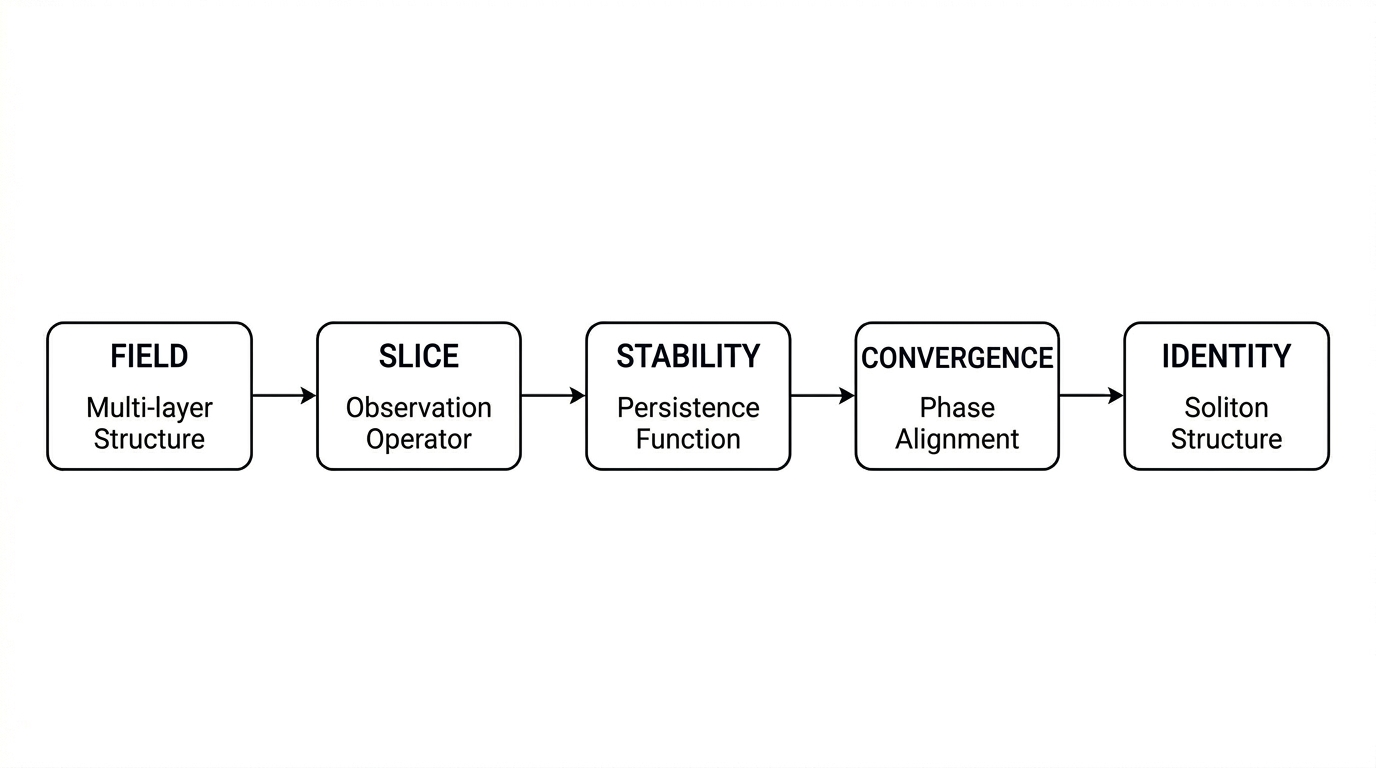
\includegraphics[width=0.82\linewidth]{figures/figure1.png}
\caption{Observation as a transformation from structure to observable representation.}
\label{fig:structure}
\end{figure}

\section{Preliminaries}

Let $\mathcal{S}$ be a category of structures and $\mathcal{X}$ a category of observations.

\subsection{Structure}

A structure is denoted by
\[
S \in \mathcal{S}.
\]

More concretely, one may write
\[
S = (E, R, \Phi),
\]
where $E$ is a set of elements, $R$ is a relational structure, and $\Phi$ is a set of constraints such as dynamics or conservation laws.

\subsection{Observation as Functor}

Observation is defined as a functor
\[
O : \mathcal{S} \to \mathcal{X}.
\]

This means that observation does not merely extract information, but maps structures and their transitions into observable representations while preserving part of their organization.

\subsection{Transitions as Morphisms}

State transitions are modeled as morphisms in $\mathcal{S}$:
\[
f : S_1 \to S_2.
\]

These morphisms may represent deformation, update, jump, or other forms of admissible transformation.

\begin{definition}[Observation]
Let $\mathcal{S}$ and $\mathcal{X}$ be categories.
An observation is a functor
\[
O : \mathcal{S} \to \mathcal{X}.
\]
\end{definition}

\section{Identity as Limit}

\begin{definition}[Identity]
Let $D : I \to \mathcal{S}$ be a diagram.
The identity under observation $O$ is defined as
\[
I_O = \lim_{\longleftarrow} (O \circ D),
\]
when the limit exists.
\end{definition}

Let
\[
D : I \to \mathcal{S}
\]
be a diagram representing the temporal evolution of structures.

Under observation, this induces the diagram
\[
O \circ D : I \to \mathcal{X}.
\]

Identity is defined as the limit of this observed diagram:
\[
I_O = \lim_{\longleftarrow} (O \circ D).
\]

The limit, when it exists, defines a universal object satisfying the commutativity of the diagram.
This expresses the idea that identity is not a static object, but the stable coherence emerging across observed structural transitions.

\begin{figure}[H]
\centering
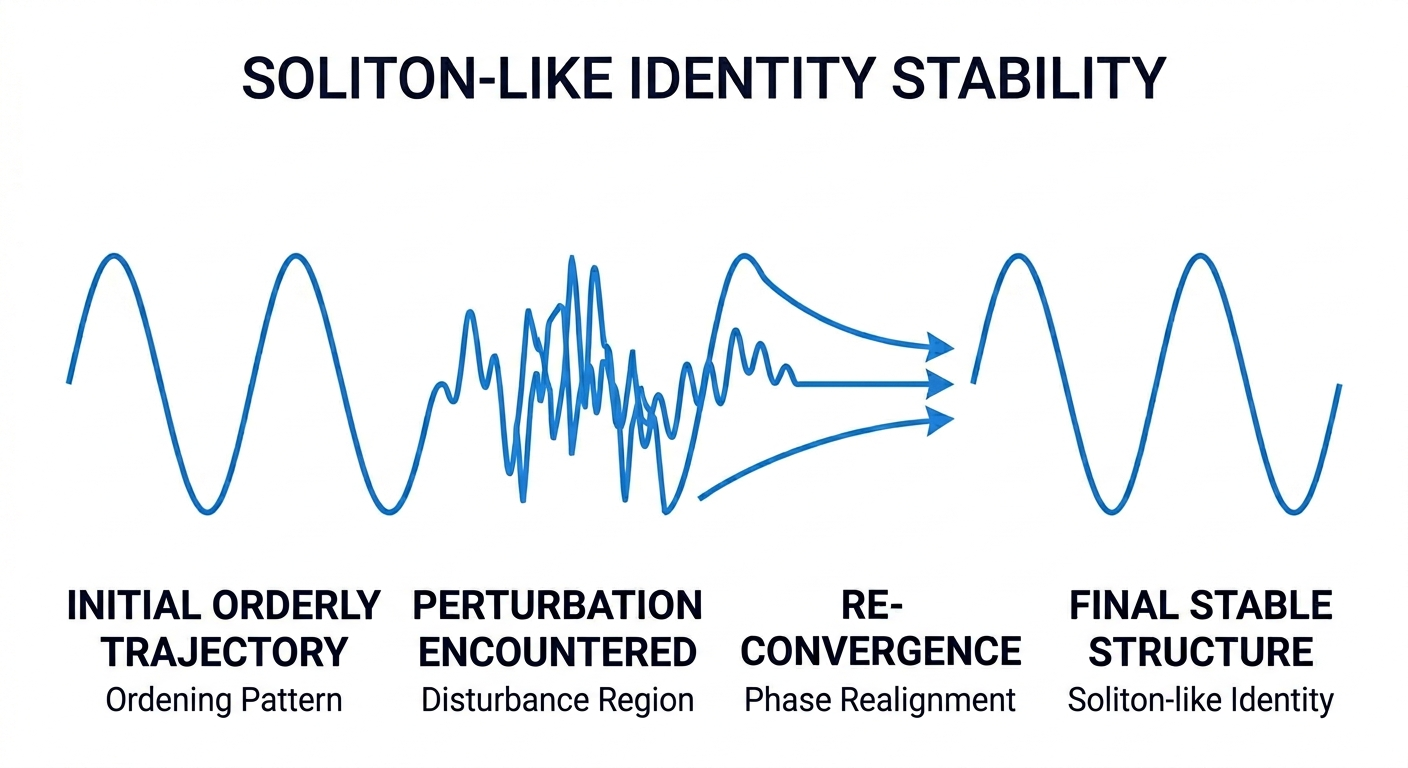
\includegraphics[width=0.82\linewidth]{figures/figure2.png}
\caption{Identity as a stability-preserving trajectory under observation.}
\label{fig:identity}
\end{figure}

In this formulation, identity is neither a frozen state nor a fixed substance. It is the limit structure that remains coherent through transformation.

\begin{theorem}[Uniqueness of Identity]
Let $D : I \to \mathcal{S}$ be a diagram and
$O : \mathcal{S} \to \mathcal{X}$ an observation functor.

If the limit
\[
I_O = \lim_{\longleftarrow} (O \circ D)
\]
exists, then it is unique up to isomorphism in $\mathcal{X}$.
\end{theorem}

This implies that identity, when it exists, is not arbitrary but uniquely determined by the observed structure.

\section{Stability}

\begin{definition}[Stability]
Let $(\mathcal{S}, \mu)$ be a measure space.
The stability of a structure $S$ under observation $O$ is defined as
\[
\mathrm{Stab}_O(S)
=
\int_{\mathcal{S}} \kappa(O(S), O(S')) d\mu(S').
\]
\end{definition}

Let $(\mathcal{S}, \mu)$ be a measure space over structures.

We define stability as
\[
\mathrm{Stab}_O(S) =
\int_{\mathcal{S}} \kappa\bigl(O(S), O(S')\bigr)\, d\mu(S'),
\]
where $\kappa$ is a similarity kernel.

A standard choice is
\[
\kappa(x,y) = e^{-\alpha d(x,y)},
\]
where $d$ is a distance function on the observation space and $\alpha > 0$ is a sensitivity parameter.

This definition captures stability as robustness over neighboring structures. 
A structure is stable when nearby perturbations still produce sufficiently similar observations.
This formulation allows stability to be interpreted as expected invariance under structural perturbations.

\begin{theorem}[Stability Preserves Identity]
Let $D : I \to \mathcal{S}$ be a diagram and $O : \mathcal{S} \to \mathcal{X}$ an observation functor.

If the limit $I_O = \lim_{\longleftarrow} (O \circ D)$ exists and

\[
\inf_{t} \mathrm{Stab}_O(S_t) > \epsilon > 0,
\]

then the identity $I_O$ is preserved under perturbations of the trajectory in expectation.
\end{theorem}

This theorem formalizes the intuition that identity emerges as a stable invariant under persistent observation.

\section{Jump and Structural Transition}

A jump is understood as a nontrivial structural transition:
\[
J : S_t \to S_{t+1}.
\]

Unlike smooth local updates, a jump may correspond to discontinuity in representation while still preserving higher-order coherence.

\begin{figure}[H]
\centering
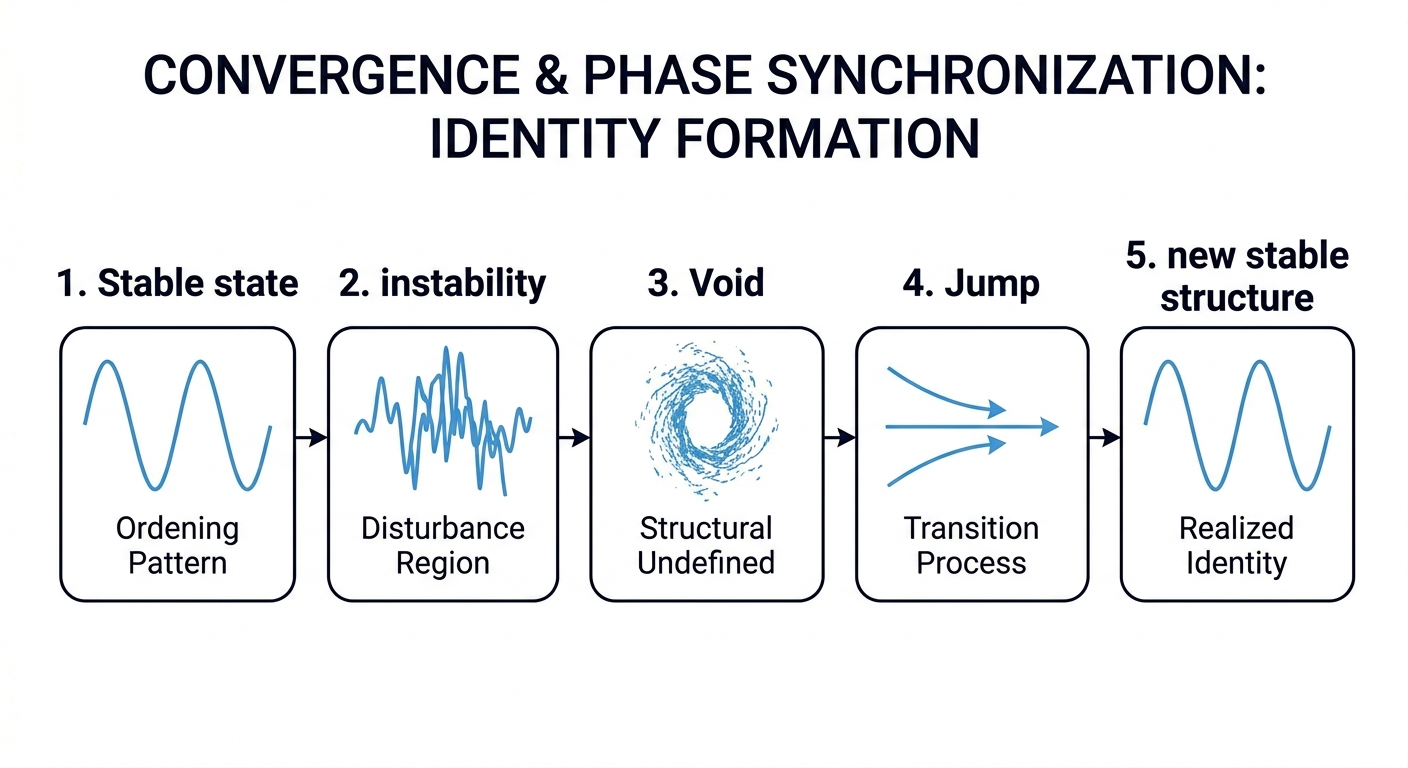
\includegraphics[width=0.82\linewidth]{figures/figure3.png}
\caption{Structural transition through instability and jump.}
\label{fig:jump}
\end{figure}

The Gyro Logic interpretation is that instability is not merely failure; it is also the generative condition for transition into a new stable regime.

\section{Unified System}

The conceptual flow of the system can be summarized as:
\[
S \rightarrow O(S) \rightarrow \mathrm{Stab} \rightarrow I_O \rightarrow \text{Self / higher integration}.
\]

This means that structure becomes observable through functorial transformation, stability evaluates persistence under perturbation, and identity emerges as a higher-order coherence over time.

\begin{figure}[H]
\centering

\includegraphics[width=0.82\linewidth]{figures/figure4.png}
\caption{Recursive structure of the Gyro Logic system.}
\label{fig:system}
\end{figure}

This recursive loop suggests that observation and structure are mutually defining processes.
The recursive nature of the framework allows observation and structure to co-determine one another through repeated transformation and evaluation.
This mutual dependency is a key feature distinguishing Gyro Logic from classical static frameworks.

\section{Consciousness as Instability Traversal}

Within the broader Gyro Logic framework, consciousness may be interpreted as the capacity to detect, hold, and resolve instability.

This can be schematically understood as:
\[
\text{Detect} \rightarrow \text{Hold} \rightarrow \text{Resolve} \rightarrow \text{Jump}.
\]

\begin{figure}[H]
\centering
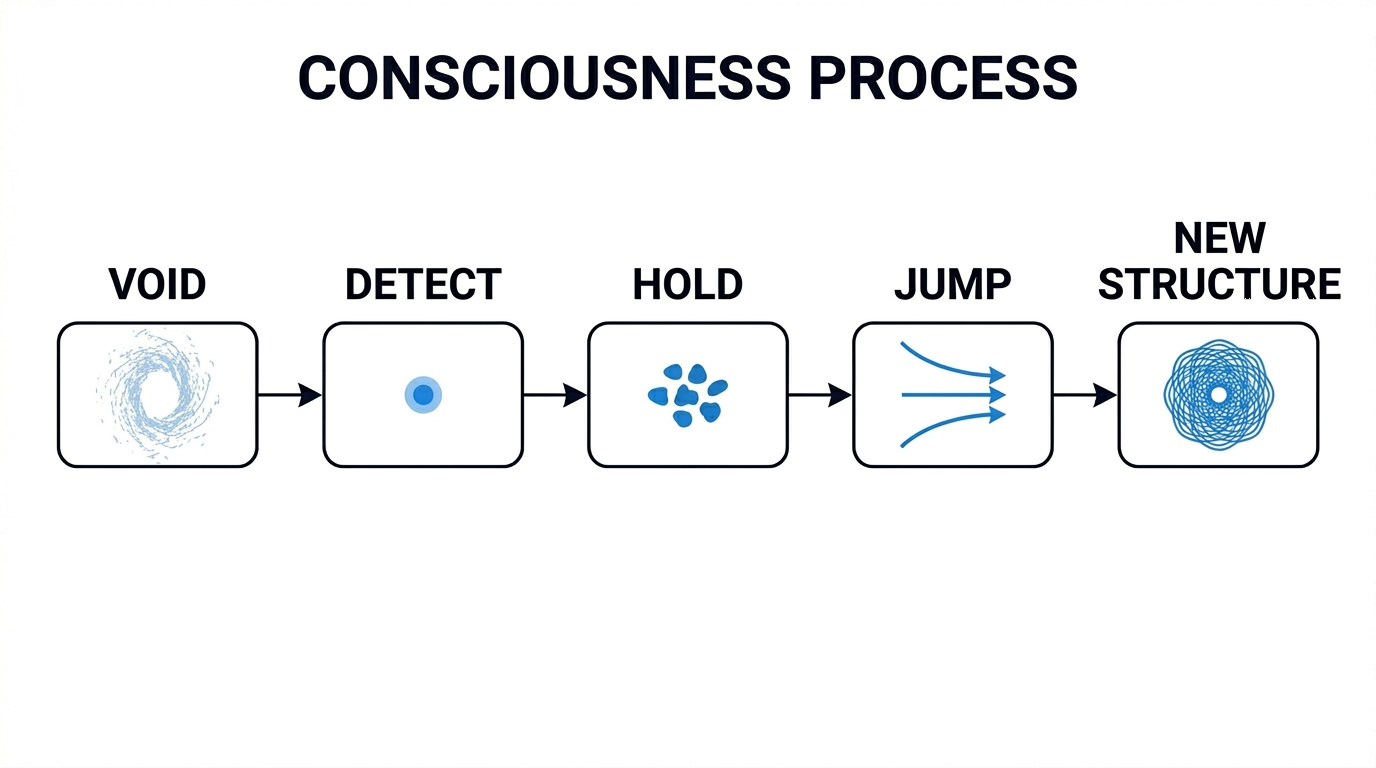
\includegraphics[width=0.82\linewidth]{figures/figure5.png}
\caption{Consciousness as the ability to traverse instability.}
\label{fig:consciousness}
\end{figure}

This interpretation does not reduce consciousness to static representation, but associates it with dynamic passage through unstable regimes.

\section{Self as Integration of Identities}

Let $\{I_1, I_2, \dots, I_n\}$ denote multiple identity structures formed across scales or episodes.

Then self may be interpreted as their temporal and structural integration:
\[
\mathrm{Self} = \mathcal{I}(I_1, I_2, \dots, I_n),
\]
where $\mathcal{I}$ denotes an integration operator.

\begin{figure}[H]
\centering
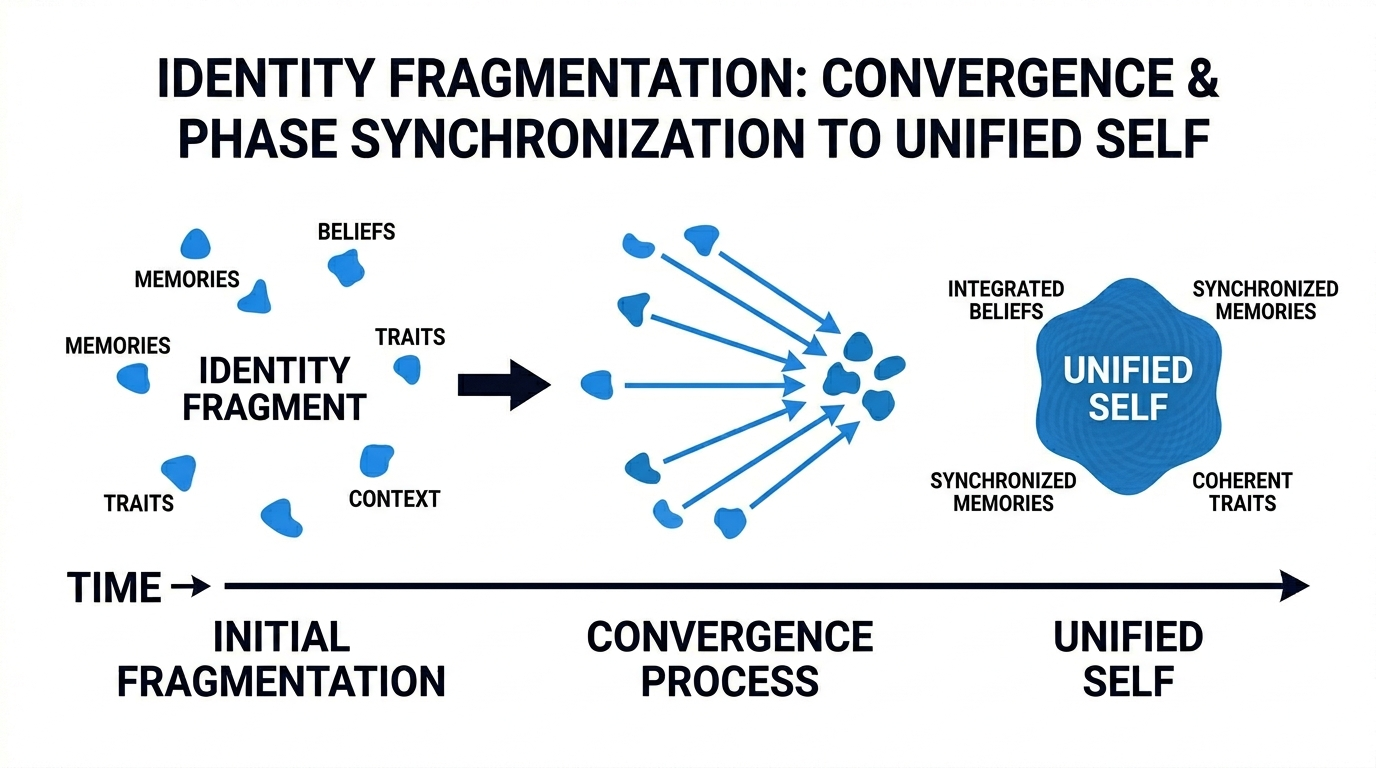
\includegraphics[width=0.82\linewidth]{figures/figure6.png}
\caption{Self as integration of identity structures over time.}
\label{fig:self}
\end{figure}

Thus, self is not identical with any one local identity, but with an organized integration across them.

\section{Time}

Time is defined as an ordered sequence of stability-preserving transitions:
\[
S_0 \to S_1 \to S_2 \to \cdots
\]

A temporal ordering is admitted when a transition retains sufficient coherence:
\[
t_1 < t_2 \iff \mathrm{Stab}(S_1 \to S_2) > \theta.
\]

This implies that time is not fundamentally continuous in itself, but emerges as a valid sequence of transitions.

\section{Inference}

\begin{proposition}[Inference as Stability Maximization]
Let $S \in \mathcal{S}$.

Inference defined by
\[
\mathrm{Inference}
=
\arg\max_{O,J}
\mathrm{Stab}_O\bigl(O(J(S))\bigr)
\]
selects transitions and observations that maximize structural stability.

In particular, inference tends to select trajectories that converge toward stable identity structures.
\end{proposition}

This establishes inference as a process guided by stability toward identity formation.

Inference is formulated as joint optimization of observation and transition:

\begin{equation}
\mathrm{Inference}
=
\arg\max_{O,J}
\mathrm{Stab}_O\bigl(O(J(S))\bigr)
\end{equation}

This redefines inference not as symbolic derivation alone, but as stability-seeking transformation under observation.

\section{Theoretical Implications}

The framework unifies several perspectives:

\begin{itemize}
  \item dynamical systems: through evolving structures and transitions,
  \item information theory: through robustness and observation,
  \item category theory: through functors, morphisms, and limits,
  \item measure theory: through stability as integrated persistence.
\end{itemize}

A key consequence is that identity becomes a mathematically expressible emergent coherence rather than a primitive assumption.

\section{Conclusion}

Gyro Logic provides a formal foundation for modeling structure, observation, stability, identity, and higher-order integration.

By combining category theory and measure theory, it reframes identity as limit, observation as functor, and stability as robustness over neighboring structures.

This offers a unified pathway connecting theory, computation, and future implementations such as GyroOS and GyroAuth.

This formulation opens a path toward computational implementations such as GyroOS and GyroAuth.

\end{document}